\documentclass[twoside]{book}

% Packages required by doxygen
\usepackage{fixltx2e}
\usepackage{calc}
\usepackage{doxygen}
\usepackage[export]{adjustbox} % also loads graphicx
\usepackage{graphicx}
\usepackage[utf8]{inputenc}
\usepackage{makeidx}
\usepackage{multicol}
\usepackage{multirow}
\PassOptionsToPackage{warn}{textcomp}
\usepackage{textcomp}
\usepackage[nointegrals]{wasysym}
\usepackage[table]{xcolor}

% Font selection
\usepackage[T1]{fontenc}
\usepackage[scaled=.90]{helvet}
\usepackage{courier}
\usepackage{amssymb}
\usepackage{sectsty}
\renewcommand{\familydefault}{\sfdefault}
\allsectionsfont{%
  \fontseries{bc}\selectfont%
  \color{darkgray}%
}
\renewcommand{\DoxyLabelFont}{%
  \fontseries{bc}\selectfont%
  \color{darkgray}%
}
\newcommand{\+}{\discretionary{\mbox{\scriptsize$\hookleftarrow$}}{}{}}

% Page & text layout
\usepackage{geometry}
\geometry{%
  a4paper,%
  top=2.5cm,%
  bottom=2.5cm,%
  left=2.5cm,%
  right=2.5cm%
}
\tolerance=750
\hfuzz=15pt
\hbadness=750
\setlength{\emergencystretch}{15pt}
\setlength{\parindent}{0cm}
\setlength{\parskip}{3ex plus 2ex minus 2ex}
\makeatletter
\renewcommand{\paragraph}{%
  \@startsection{paragraph}{4}{0ex}{-1.0ex}{1.0ex}{%
    \normalfont\normalsize\bfseries\SS@parafont%
  }%
}
\renewcommand{\subparagraph}{%
  \@startsection{subparagraph}{5}{0ex}{-1.0ex}{1.0ex}{%
    \normalfont\normalsize\bfseries\SS@subparafont%
  }%
}
\makeatother

% Headers & footers
\usepackage{fancyhdr}
\pagestyle{fancyplain}
\fancyhead[LE]{\fancyplain{}{\bfseries\thepage}}
\fancyhead[CE]{\fancyplain{}{}}
\fancyhead[RE]{\fancyplain{}{\bfseries\leftmark}}
\fancyhead[LO]{\fancyplain{}{\bfseries\rightmark}}
\fancyhead[CO]{\fancyplain{}{}}
\fancyhead[RO]{\fancyplain{}{\bfseries\thepage}}
\fancyfoot[LE]{\fancyplain{}{}}
\fancyfoot[CE]{\fancyplain{}{}}
\fancyfoot[RE]{\fancyplain{}{\bfseries\scriptsize Generated by Doxygen }}
\fancyfoot[LO]{\fancyplain{}{\bfseries\scriptsize Generated by Doxygen }}
\fancyfoot[CO]{\fancyplain{}{}}
\fancyfoot[RO]{\fancyplain{}{}}
\renewcommand{\footrulewidth}{0.4pt}
\renewcommand{\chaptermark}[1]{%
  \markboth{#1}{}%
}
\renewcommand{\sectionmark}[1]{%
  \markright{\thesection\ #1}%
}

% Indices & bibliography
\usepackage{natbib}
\usepackage[titles]{tocloft}
\setcounter{tocdepth}{3}
\setcounter{secnumdepth}{5}
\makeindex

% Hyperlinks (required, but should be loaded last)
\usepackage{ifpdf}
\ifpdf
  \usepackage[pdftex,pagebackref=true]{hyperref}
\else
  \usepackage[ps2pdf,pagebackref=true]{hyperref}
\fi
\hypersetup{%
  colorlinks=true,%
  linkcolor=blue,%
  citecolor=blue,%
  unicode%
}

% Custom commands
\newcommand{\clearemptydoublepage}{%
  \newpage{\pagestyle{empty}\cleardoublepage}%
}

\usepackage{caption}
\captionsetup{labelsep=space,justification=centering,font={bf},singlelinecheck=off,skip=4pt,position=top}

%===== C O N T E N T S =====

\begin{document}

% Titlepage & ToC
\hypersetup{pageanchor=false,
             bookmarksnumbered=true,
             pdfencoding=unicode
            }
\pagenumbering{alph}
\begin{titlepage}
\vspace*{7cm}
\begin{center}%
{\Large Lenora OS }\\
\vspace*{1cm}
{\large Generated by Doxygen 1.8.14}\\
\end{center}
\end{titlepage}
\clearemptydoublepage
\pagenumbering{roman}
\tableofcontents
\clearemptydoublepage
\pagenumbering{arabic}
\hypersetup{pageanchor=true}

%--- Begin generated contents ---
\chapter{Hierarchical Index}
\section{Class Hierarchy}
This inheritance list is sorted roughly, but not completely, alphabetically\+:\begin{DoxyCompactList}
\item \contentsline{section}{lenora\+:\+:Global\+Descriptor\+Table}{\pageref{classlenora_1_1GlobalDescriptorTable}}{}
\item Keyboard\+Event\+Handler\begin{DoxyCompactList}
\item \contentsline{section}{Print\+Keyboard\+Event\+Handler}{\pageref{classPrintKeyboardEventHandler}}{}
\end{DoxyCompactList}
\item Mouse\+Event\+Handler\begin{DoxyCompactList}
\item \contentsline{section}{Console\+Mouse}{\pageref{classConsoleMouse}}{}
\end{DoxyCompactList}
\item \contentsline{section}{lenora\+:\+:Global\+Descriptor\+Table\+:\+:Segment\+Descriptor}{\pageref{classlenora_1_1GlobalDescriptorTable_1_1SegmentDescriptor}}{}
\end{DoxyCompactList}

\chapter{Class Index}
\section{Class List}
Here are the classes, structs, unions and interfaces with brief descriptions\+:\begin{DoxyCompactList}
\item\contentsline{section}{\hyperlink{classConsoleMouse}{Console\+Mouse} }{\pageref{classConsoleMouse}}{}
\item\contentsline{section}{\hyperlink{classlenora_1_1GlobalDescriptorTable}{lenora\+::\+Global\+Descriptor\+Table} }{\pageref{classlenora_1_1GlobalDescriptorTable}}{}
\item\contentsline{section}{\hyperlink{classPrintKeyboardEventHandler}{Print\+Keyboard\+Event\+Handler} }{\pageref{classPrintKeyboardEventHandler}}{}
\item\contentsline{section}{\hyperlink{classlenora_1_1GlobalDescriptorTable_1_1SegmentDescriptor}{lenora\+::\+Global\+Descriptor\+Table\+::\+Segment\+Descriptor} }{\pageref{classlenora_1_1GlobalDescriptorTable_1_1SegmentDescriptor}}{}
\end{DoxyCompactList}

\chapter{Class Documentation}
\hypertarget{classConsoleMouse}{}\section{Console\+Mouse Class Reference}
\label{classConsoleMouse}\index{Console\+Mouse@{Console\+Mouse}}
Inheritance diagram for Console\+Mouse\+:\begin{figure}[H]
\begin{center}
\leavevmode
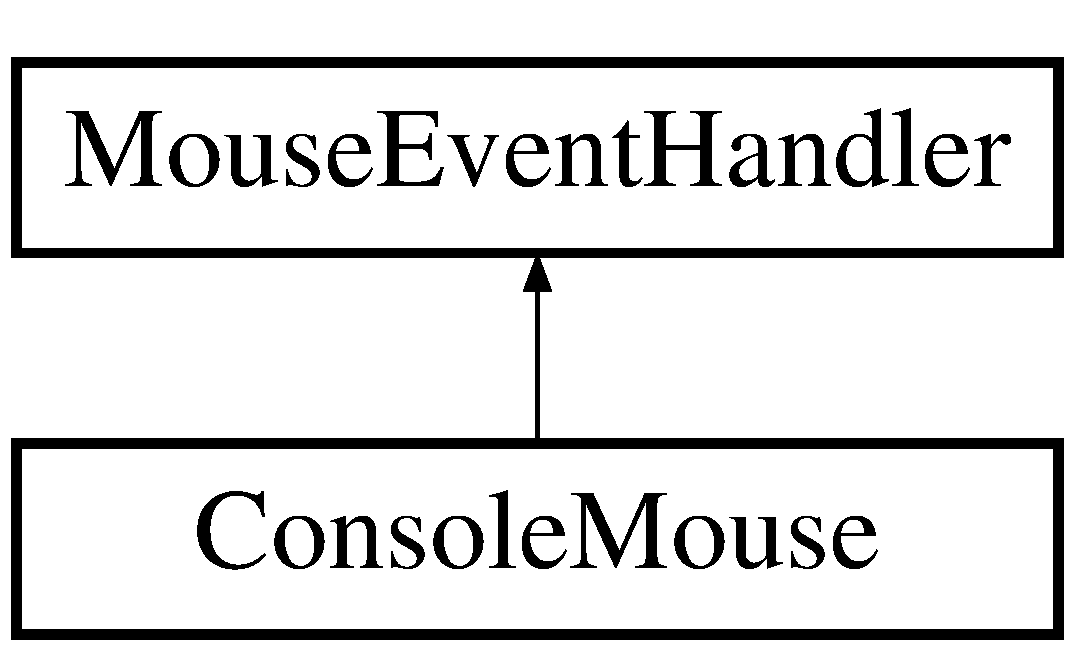
\includegraphics[height=2.000000cm]{classConsoleMouse}
\end{center}
\end{figure}
\subsection*{Public Member Functions}
\begin{DoxyCompactItemize}
\item 
\mbox{\Hypertarget{classConsoleMouse_ad3b3c7cf5eed05fb369ae4f0f018eb6c}\label{classConsoleMouse_ad3b3c7cf5eed05fb369ae4f0f018eb6c}} 
virtual void {\bfseries On\+Mouse\+Activate} ()
\item 
\mbox{\Hypertarget{classConsoleMouse_a8d48f2e512994c819f9ad0a317ac213e}\label{classConsoleMouse_a8d48f2e512994c819f9ad0a317ac213e}} 
virtual void {\bfseries On\+Mouse\+Down} (uint8\+\_\+t button)
\item 
\mbox{\Hypertarget{classConsoleMouse_a33a6f1e0c759b0964536d6204196b225}\label{classConsoleMouse_a33a6f1e0c759b0964536d6204196b225}} 
virtual void {\bfseries On\+Mouse\+Up} (uint8\+\_\+t button)
\item 
\mbox{\Hypertarget{classConsoleMouse_a36634acf764621f33ac03d6615109278}\label{classConsoleMouse_a36634acf764621f33ac03d6615109278}} 
virtual void {\bfseries On\+Mouse\+Move} (int x\+\_\+offset, int y\+\_\+offset)
\end{DoxyCompactItemize}


The documentation for this class was generated from the following file\+:\begin{DoxyCompactItemize}
\item 
/home/zorro/github/\+Lenora\+O\+S/src/kernel.\+cpp\end{DoxyCompactItemize}

\hypertarget{classlenora_1_1GlobalDescriptorTable}{}\section{lenora\+:\+:Global\+Descriptor\+Table Class Reference}
\label{classlenora_1_1GlobalDescriptorTable}\index{lenora\+::\+Global\+Descriptor\+Table@{lenora\+::\+Global\+Descriptor\+Table}}
\subsection*{Classes}
\begin{DoxyCompactItemize}
\item 
class \hyperlink{classlenora_1_1GlobalDescriptorTable_1_1SegmentDescriptor}{Segment\+Descriptor}
\end{DoxyCompactItemize}
\subsection*{Public Member Functions}
\begin{DoxyCompactItemize}
\item 
\mbox{\Hypertarget{classlenora_1_1GlobalDescriptorTable_ad08f49a5cb263c7fb7c559798b6b4901}\label{classlenora_1_1GlobalDescriptorTable_ad08f49a5cb263c7fb7c559798b6b4901}} 
class \hyperlink{classlenora_1_1GlobalDescriptorTable_1_1SegmentDescriptor}{lenora\+::\+Global\+Descriptor\+Table\+::\+Segment\+Descriptor} {\bfseries \+\_\+\+\_\+attribute\+\_\+\+\_\+} ((packed))
\item 
\mbox{\Hypertarget{classlenora_1_1GlobalDescriptorTable_a97d81f058e0d5a49713ad4894be23ae8}\label{classlenora_1_1GlobalDescriptorTable_a97d81f058e0d5a49713ad4894be23ae8}} 
lenora\+::common\+::uint16\+\_\+t {\bfseries Code\+Segment\+Selector} ()
\item 
\mbox{\Hypertarget{classlenora_1_1GlobalDescriptorTable_a402918f857a5f58b35097d4d36e278fd}\label{classlenora_1_1GlobalDescriptorTable_a402918f857a5f58b35097d4d36e278fd}} 
lenora\+::common\+::uint16\+\_\+t {\bfseries Data\+Segment\+Selector} ()
\end{DoxyCompactItemize}
\subsection*{Public Attributes}
\begin{DoxyCompactItemize}
\item 
\mbox{\Hypertarget{classlenora_1_1GlobalDescriptorTable_a5c2929e7d8411e0701eef53d3d78d2ad}\label{classlenora_1_1GlobalDescriptorTable_a5c2929e7d8411e0701eef53d3d78d2ad}} 
\hyperlink{classlenora_1_1GlobalDescriptorTable_1_1SegmentDescriptor}{Segment\+Descriptor} {\bfseries null\+Segment\+Selector}
\item 
\mbox{\Hypertarget{classlenora_1_1GlobalDescriptorTable_a81d7f4a8c5493e8138d4d2311ebb5513}\label{classlenora_1_1GlobalDescriptorTable_a81d7f4a8c5493e8138d4d2311ebb5513}} 
\hyperlink{classlenora_1_1GlobalDescriptorTable_1_1SegmentDescriptor}{Segment\+Descriptor} {\bfseries unused\+Segment\+Selector}
\item 
\mbox{\Hypertarget{classlenora_1_1GlobalDescriptorTable_aa236fad95318a712db0fb8dbf0e2e47b}\label{classlenora_1_1GlobalDescriptorTable_aa236fad95318a712db0fb8dbf0e2e47b}} 
\hyperlink{classlenora_1_1GlobalDescriptorTable_1_1SegmentDescriptor}{Segment\+Descriptor} {\bfseries code\+Segment\+Selector}
\item 
\mbox{\Hypertarget{classlenora_1_1GlobalDescriptorTable_a146dd72b7f1730d1b3e93da63be976ac}\label{classlenora_1_1GlobalDescriptorTable_a146dd72b7f1730d1b3e93da63be976ac}} 
\hyperlink{classlenora_1_1GlobalDescriptorTable_1_1SegmentDescriptor}{Segment\+Descriptor} {\bfseries data\+Segment\+Selector}
\end{DoxyCompactItemize}


The documentation for this class was generated from the following files\+:\begin{DoxyCompactItemize}
\item 
/home/zorro/github/\+Lenora\+O\+S/include/gdt.\+h\item 
/home/zorro/github/\+Lenora\+O\+S/src/gdt.\+cpp\end{DoxyCompactItemize}

\hypertarget{classPrintKeyboardEventHandler}{}\section{Print\+Keyboard\+Event\+Handler Class Reference}
\label{classPrintKeyboardEventHandler}\index{Print\+Keyboard\+Event\+Handler@{Print\+Keyboard\+Event\+Handler}}
Inheritance diagram for Print\+Keyboard\+Event\+Handler\+:\begin{figure}[H]
\begin{center}
\leavevmode
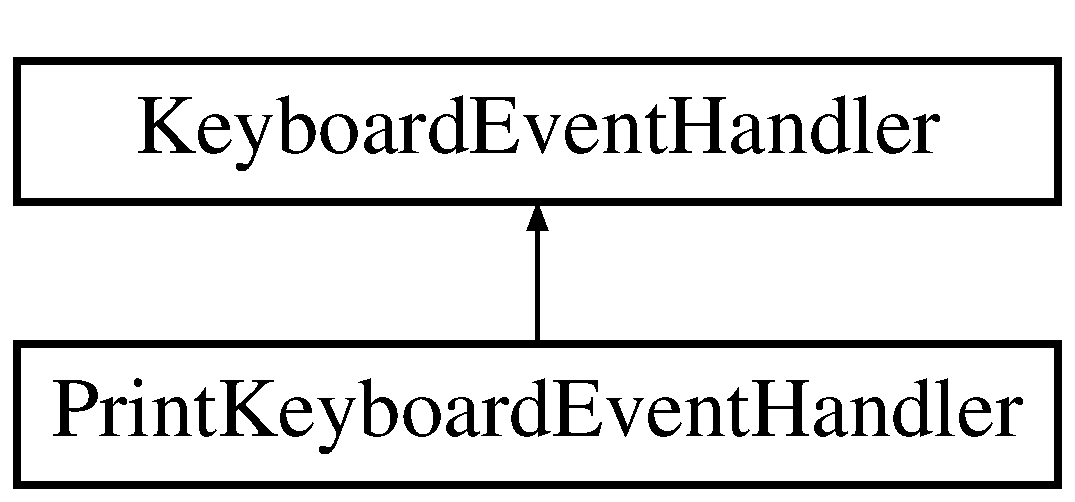
\includegraphics[height=2.000000cm]{classPrintKeyboardEventHandler}
\end{center}
\end{figure}
\subsection*{Public Member Functions}
\begin{DoxyCompactItemize}
\item 
\mbox{\Hypertarget{classPrintKeyboardEventHandler_a6f529d75127cb52467587c8efc347d98}\label{classPrintKeyboardEventHandler_a6f529d75127cb52467587c8efc347d98}} 
virtual void {\bfseries On\+Key\+Down} (char c)
\end{DoxyCompactItemize}


The documentation for this class was generated from the following file\+:\begin{DoxyCompactItemize}
\item 
/home/zorro/github/\+Lenora\+O\+S/src/kernel.\+cpp\end{DoxyCompactItemize}

\hypertarget{classlenora_1_1GlobalDescriptorTable_1_1SegmentDescriptor}{}\section{lenora\+:\+:Global\+Descriptor\+Table\+:\+:Segment\+Descriptor Class Reference}
\label{classlenora_1_1GlobalDescriptorTable_1_1SegmentDescriptor}\index{lenora\+::\+Global\+Descriptor\+Table\+::\+Segment\+Descriptor@{lenora\+::\+Global\+Descriptor\+Table\+::\+Segment\+Descriptor}}
\subsection*{Public Member Functions}
\begin{DoxyCompactItemize}
\item 
\mbox{\Hypertarget{classlenora_1_1GlobalDescriptorTable_1_1SegmentDescriptor_a42f4dce4bce5aaa4a70cb7748daaf2d8}\label{classlenora_1_1GlobalDescriptorTable_1_1SegmentDescriptor_a42f4dce4bce5aaa4a70cb7748daaf2d8}} 
{\bfseries Segment\+Descriptor} (lenora\+::common\+::uint32\+\_\+t base, lenora\+::common\+::uint32\+\_\+t limit, lenora\+::common\+::uint8\+\_\+t type)
\item 
\mbox{\Hypertarget{classlenora_1_1GlobalDescriptorTable_1_1SegmentDescriptor_aeb065fd3ef4a652e8fab35bd5b0b4a53}\label{classlenora_1_1GlobalDescriptorTable_1_1SegmentDescriptor_aeb065fd3ef4a652e8fab35bd5b0b4a53}} 
lenora\+::common\+::uint32\+\_\+t {\bfseries Base} ()
\item 
\mbox{\Hypertarget{classlenora_1_1GlobalDescriptorTable_1_1SegmentDescriptor_a35d53521838d776e8250bbb07e3f5be4}\label{classlenora_1_1GlobalDescriptorTable_1_1SegmentDescriptor_a35d53521838d776e8250bbb07e3f5be4}} 
lenora\+::common\+::uint32\+\_\+t {\bfseries Limit} ()
\end{DoxyCompactItemize}


The documentation for this class was generated from the following files\+:\begin{DoxyCompactItemize}
\item 
/home/zorro/github/\+Lenora\+O\+S/include/gdt.\+h\item 
/home/zorro/github/\+Lenora\+O\+S/src/gdt.\+cpp\end{DoxyCompactItemize}

%--- End generated contents ---

% Index
\backmatter
\newpage
\phantomsection
\clearemptydoublepage
\addcontentsline{toc}{chapter}{Index}
\printindex

\end{document}
